\chapter{Risultati sperimentali}
\vskip 1cm

\textit{In questo capitolo vengono discussi i risultati sperimentali, seguendo la procedura di valutazione introdotta nel capitolo precedente, relativi a GNINA ed AutoDock Vina come software di docking computazionale. Inoltre, vengono discusse le differenze tra i software di docking utilizzati in termini di risultati ed interazioni osservate. }

\vskip 1cm
\section{Riepilogo dell'esperimento}
A titolo d'esempio, sono riportate le prestazioni di blind docking relative ad esperimenti di docking proteina-ligando. Rispetto al dataset iniziale, composto da strutture molecolari di proteine e ligandi, sono stati selezionati solo alcuni dei risultati del docking molecolare. 
Le proteine (e quindi i risultati del docking selezionati) sono state assortite in maniera tale da ottenere una certa varietà di dati di analisi. Ricordo che il dataset iniziale, è stato sottoposto alla procedura di preparazione, mostrata nella Sezione \ref{preparation}.
I risultati del docking sono stati poi valutati in termini di tempi d'esecuzione, RMSD delle pose, contatti, legami ed affinità risultanti, come illustrato dalla procedura di valutazione nella Sezione \ref{evalutation}.

Per fornire una visione più ampia e chiara delle prestazioni del software GNINA, in cui la rete neurale convoluzionale è stata utilizzata nella fase di \textit{"rescore"}, sono stati considerati i risultati prodotti da AutoDock Vina, un software ampiamente utilizzato negli esperimenti di blind docking, applicando le medesime procedure di preparazione e di valutazione rispettivamente al dataset iniziale ed ai risultati prodotti. 

Le prestazioni sono state riportate a vari livelli di profondità, partendo da una prima considerazione visuale della posa del ligando predetta, arrivando a motivare e valutare i valori osservati per le caratteristiche riportate. 

Le proteine selezionate per l'analisi dei risultati del docking effettuato tra i due software sopracitati sono le proteine 1FCU, 2H8V, 3FE9, 4E81, 5XZ3\_A e 6LQK\_B.

\section{Visualizzazione della predizione della posa}

Sono mostrate alcune conformazioni proteina-ligando relativamente all'esperimento di single docking tra proteine di dimensioni differenti (2H8V, 4E81, 6LQK\_B) ed alcuni dei ligandi del dataset iniziale (Acrinathrin, Dimethomorph, Glyphosate e Oxyfluorfen).

Lo scopo della visualizzazione di questi complessi è quello di avere una visione generale, nei limiti del possibile, delle predizioni effettuate da GNINA ed ovviamente valutarne le differenze rispetto a quelle di AutoDock Vina. Inoltre, è interessante osservare la differenza delle pose predette tra i suddetti software all'aumentare delle dimensioni della proteina.

Ai fini della visualizzazione delle strutture, è stato utilizzato AutoDockTools, introdotto nella Sezione \ref{autodocktools}.
Relativamente alla proteina viene mostrata direttamente la sua struttura molecolare. in quanto di seconda importanza rispetto alle pose predette dei ligandi di cui invece viene mostrata la superficie, per portare all'attenzione la porzione di immagine a cui siamo interessati.

Viene sottolineato che è visualizzata solo la posa migliore predetta da ciascun software, motivo per cui è possibile che un'eventuale differenza della predizione sia dettata dalla differenza dei criteri utilizzati, da eventuali filtri applicati (ad esempio sull'RMSD) e dal seme casuale generato ad ogni esecuzione del docking.

\begin{figure}[H]
    \centering
    \begin{subfigure}[b]{0.475\textwidth}
        \centering
        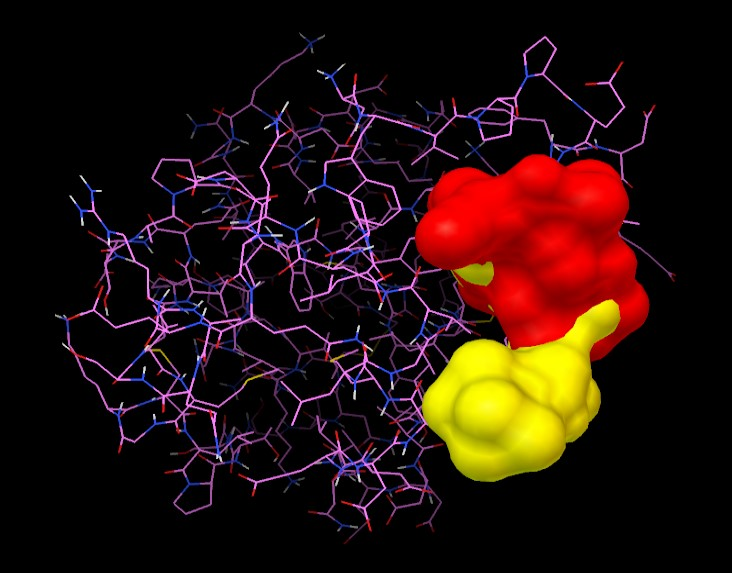
\includegraphics[width=\textwidth, height=6cm]{images/chapter4/visualization/2h8v_acrinathrin.jpg}
        \caption[]%
        {{\small Acrinathrin}}    
        \label{fig:2h8v_acrinathrin}
    \end{subfigure}
    \hfill
    \begin{subfigure}[b]{0.475\textwidth}  
        \centering 
        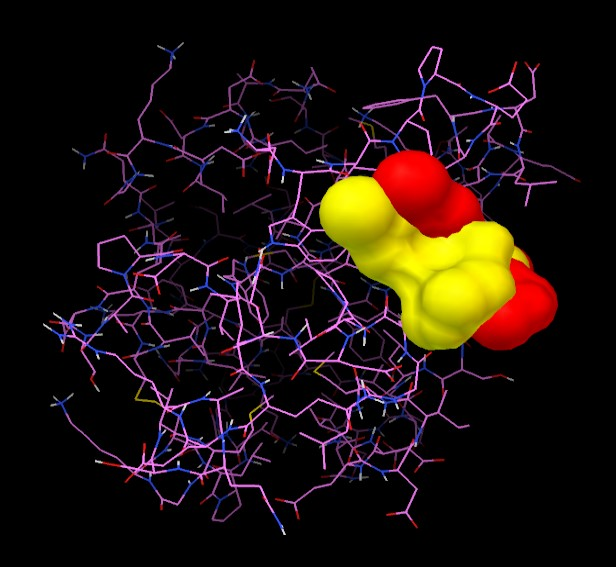
\includegraphics[width=\textwidth, height=6cm]{images/chapter4/visualization/2h8v_dimethomorph.jpg}
        \caption[]%
        {{\small Dimethomorph}}    
        \label{fig:2h8v_dimethomorph}
    \end{subfigure}
    \vskip\baselineskip
    \begin{subfigure}[b]{0.475\textwidth}   
        \centering 
        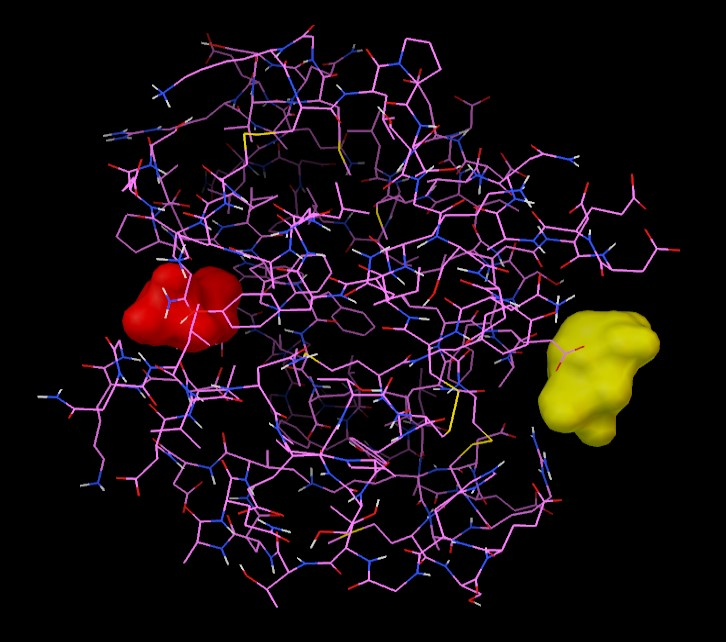
\includegraphics[width=\textwidth, height=6cm]{images/chapter4/visualization/2h8v_glyphosate.jpg}
        \caption[]%
        {{\small Glyphosate}}    
        \label{fig:2h8v_glyphosate}
    \end{subfigure}
    \hfill
    \begin{subfigure}[b]{0.475\textwidth}   
        \centering 
        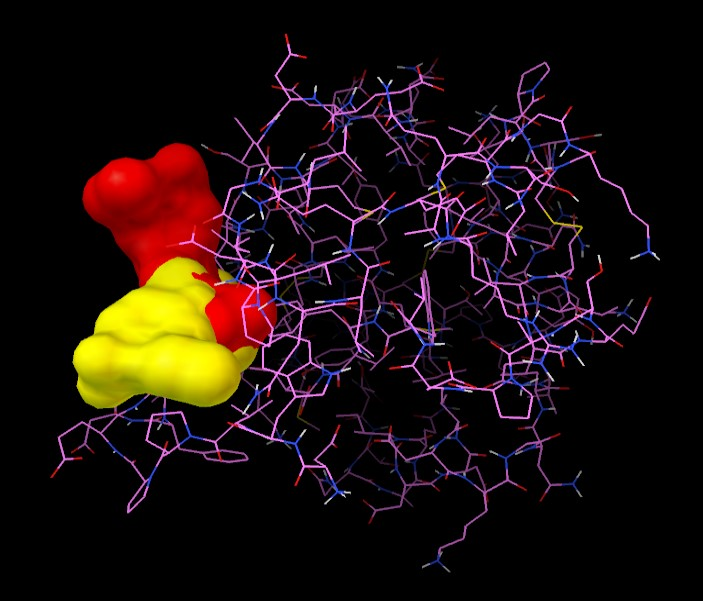
\includegraphics[width=\textwidth, height=6cm]{images/chapter4/visualization/2h8v_oxyfluorfen.jpg}
        \caption[]%
        {{\small Oxyfluorfen}}    
        \label{fig:2h8v_oxyfluorfen}
    \end{subfigure}
    \caption[Conformazioni proteina-ligando per la proteina 2H8V]
    {\small Visualizzazione delle migliori pose generate da GNINA (in giallo) ed AutoDock Vina (in rosso) relativamente alla proteina 2H8V ed alcuni dei ligandi del dataset iniziale (Acrinathrin, Dimethomorph, Glyphosate, Oxyfluorfen).} 
    \label{fig:2h8v}
\end{figure}

A partire dalla Figura \ref{fig:2h8v}, è possibile notare come, per una proteina di modeste dimensioni, tendenzialmente il sito di legame relativo alle migliori pose predette è circa lo stesso, a meno di orientazioni e torsioni del ligando coinvolto, risultando predizioni piuttosto simili tra i software, sebbene configurati per scopi diversi.


\begin{figure}
    \centering
    \begin{subfigure}[b]{0.475\textwidth}
        \centering
        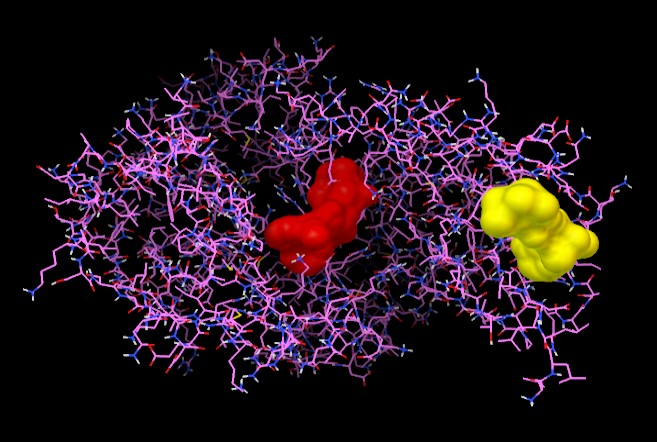
\includegraphics[width=\textwidth, height=6cm]{images/chapter4/visualization/4e81_acrinathrin.jpg}
        \caption[]%
        {{\small Acrinathrin}}    
        \label{fig:2h8v_acrinathrin}
    \end{subfigure}
    \hfill
    \begin{subfigure}[b]{0.475\textwidth}  
        \centering 
        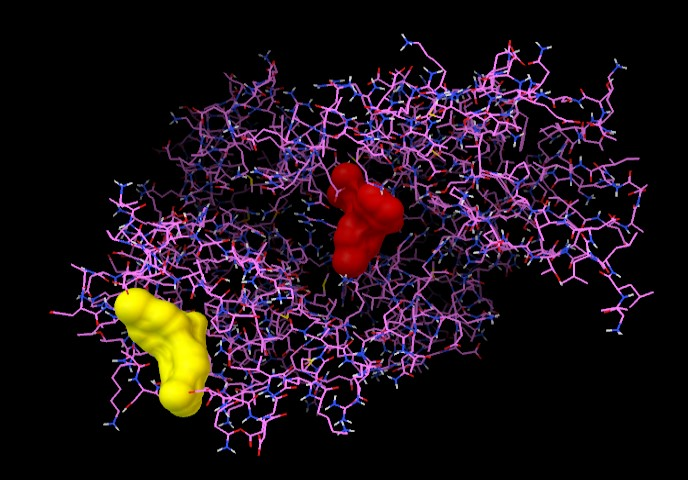
\includegraphics[width=\textwidth, height=6cm]{images/chapter4/visualization/4e81_dimethomorph.jpg}
        \caption[]%
        {{\small Dimethomorph}}    
        \label{fig:2h8v_dimethomorph}
    \end{subfigure}
    \vskip\baselineskip
    \begin{subfigure}[b]{0.475\textwidth}   
        \centering 
        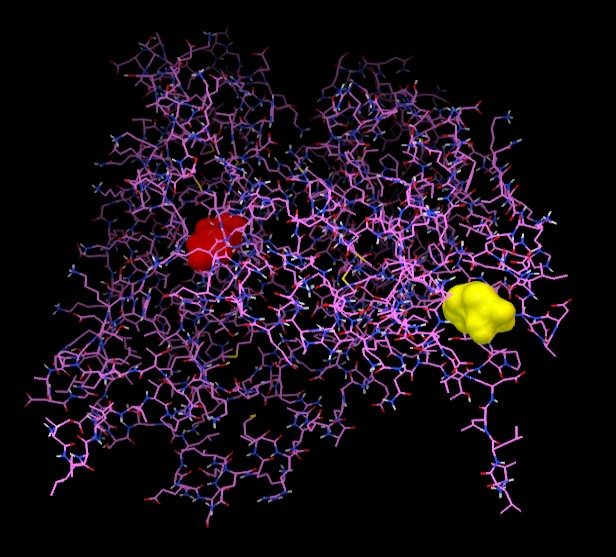
\includegraphics[width=\textwidth, height=6cm]{images/chapter4/visualization/4e81_glyphosate.jpg}
        \caption[]%
        {{\small Glyphosate}}    
        \label{fig:2h8v_glyphosate}
    \end{subfigure}
    \hfill
    \begin{subfigure}[b]{0.475\textwidth}   
        \centering 
        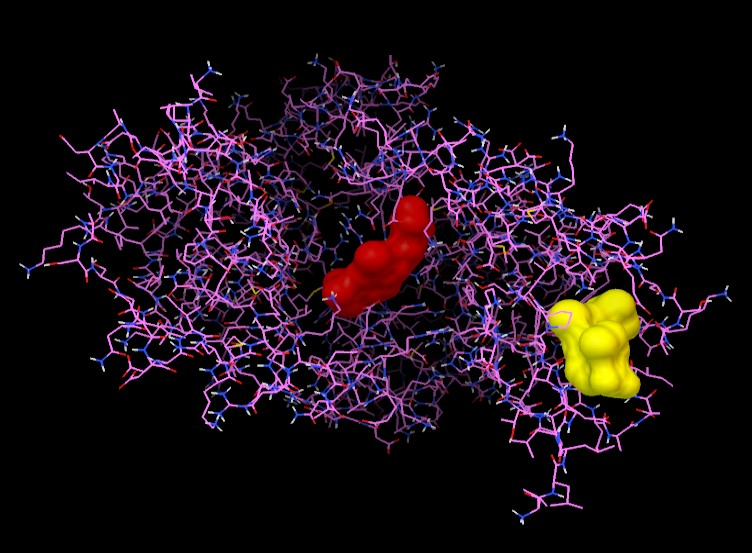
\includegraphics[width=\textwidth, height=6cm]{images/chapter4/visualization/4e81_oxyfluorfen.jpg}
        \caption[]%
        {{\small Oxyfluorfen}}    
        \label{fig:2h8v_oxyfluorfen}
    \end{subfigure}
    \caption[Conformazioni proteina-ligando per la proteina 4E81. ]
    {\small Visualizzazione delle migliori pose generate da GNINA (in giallo) ed AutoDock Vina (in rosso) relativamente alla proteina 4E81 ed alcuni dei ligandi del dataset iniziale (Acrinathrin, Dimethomorph, Glyphosate, Oxyfluorfen).} 
    \label{fig:4e81}
\end{figure}



Le cose si fanno interessanti invece se osserviamo una proteina di dimensioni maggiori rispetto alla precedente. La Figura \ref{fig:4e81} mostra la notevole differenza nelle predizioni: nel caso di GNINA, il ligando risulta occupare una posizione quasi esterna alla proteina mentre è tendenzialmente interna nel caso di AutoDock Vina. E' ipotizzabile che questa situazione sia condizionata dalla struttura molecolare della proteina coinvolta, tuttavia è comunque una differenza rispetto a strutture proteiche di questo genere.


\begin{figure}[H]
    \centering
    \begin{subfigure}[b]{0.475\textwidth}
        \centering
        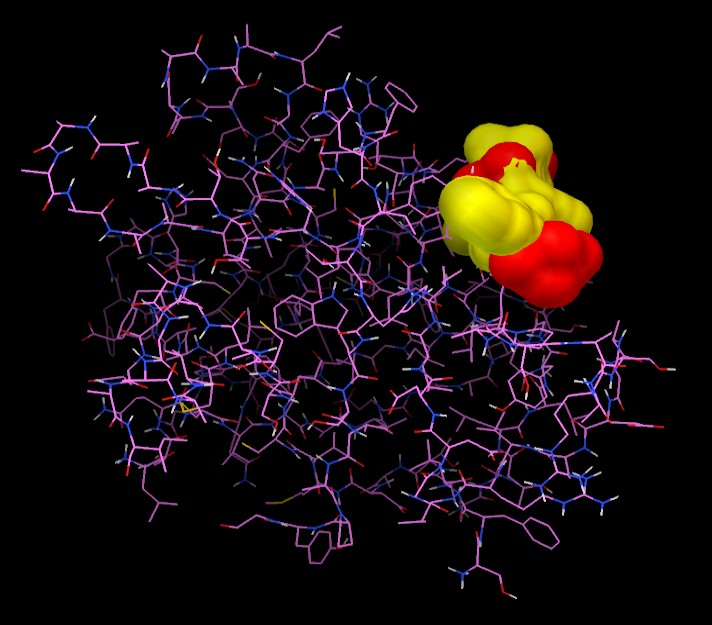
\includegraphics[width=\textwidth, height=6cm]{images/chapter4/visualization/6lqk_b_acrinathrin.jpg}
        \caption[]%
        {{\small Acrinathrin}}    
        \label{fig:2h8v_acrinathrin}
    \end{subfigure}
    \hfill
    \begin{subfigure}[b]{0.475\textwidth}  
        \centering 
        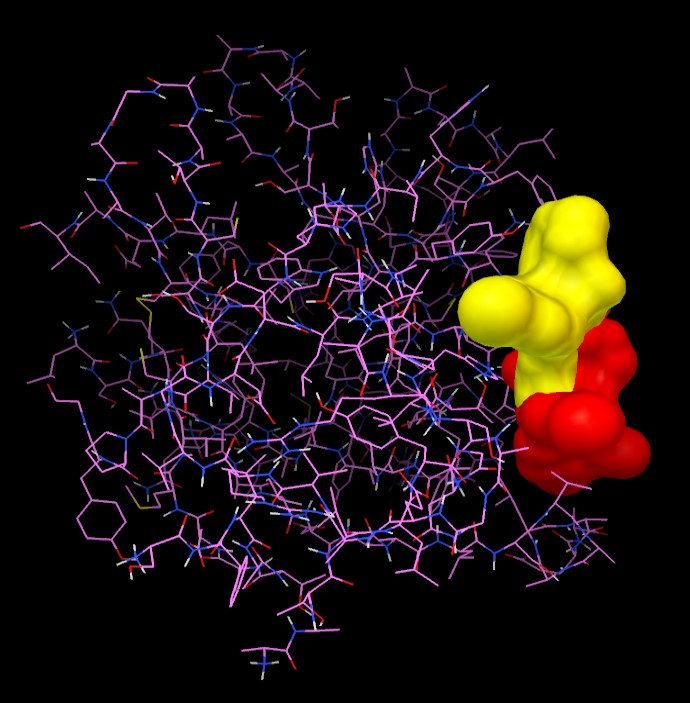
\includegraphics[width=\textwidth, height=6cm]{images/chapter4/visualization/6lqk_b_dimethomorph.jpg}
        \caption[]%
        {{\small Dimethomorph}}    
        \label{fig:2h8v_dimethomorph}
    \end{subfigure}
    \vskip\baselineskip
    \begin{subfigure}[b]{0.475\textwidth}   
        \centering 
        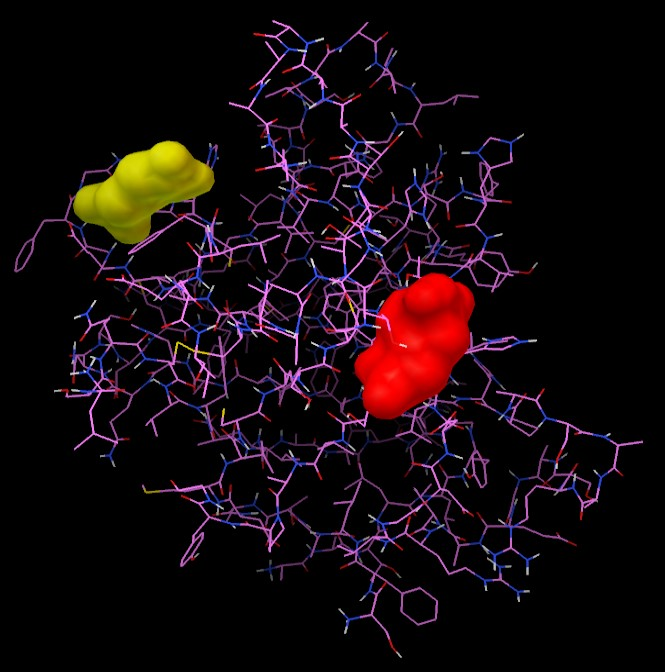
\includegraphics[width=\textwidth, height=6cm]{images/chapter4/visualization/6lqk_b_glyphosate.jpg}
        \caption[]%
        {{\small Glyphosate}}    
        \label{fig:2h8v_glyphosate}
    \end{subfigure}
    \hfill
    \begin{subfigure}[b]{0.475\textwidth}   
        \centering 
        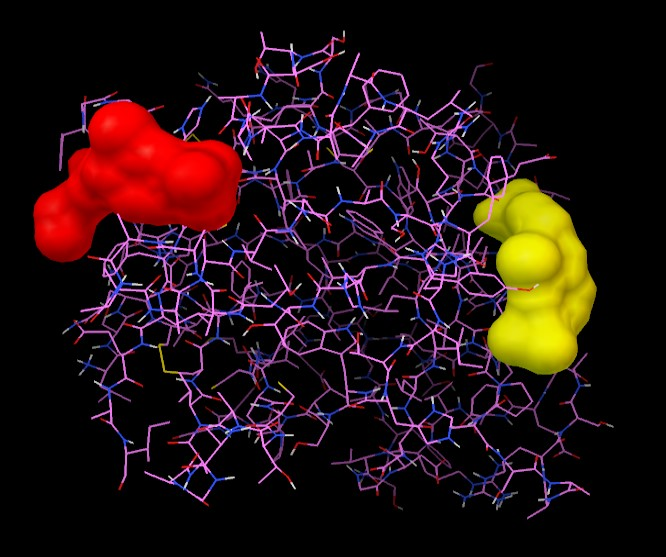
\includegraphics[width=\textwidth, height=6cm]{images/chapter4/visualization/6lqk_b_oxyfluorfen.jpg}
        \caption[]%
        {{\small Oxyfluorfen}}    
        \label{fig:2h8v_oxyfluorfen}
        \end{subfigure}
    \caption[Conformazioni proteina-ligando per la proteina 6LQK\_B. ]
    {\small Visualizzazione delle migliori pose generate da GNINA (in giallo) ed AutoDock Vina (in rosso) relativamente alla proteina 6LQK\_B ed alcuni dei ligandi del dataset iniziale (Acrinathrin, Dimethomorph, Glyphosate, Oxyfluorfen).} 
    \label{fig:6lqk_b}
\end{figure}

L'ultima visualizzazione riguarda la proteina più grande delle tre sopracitate ossia la 6LQK\_B. La Figura \ref{fig:6lqk_b} mostra come coesistono situazioni in cui la predizione è circa la stessa ed altre in cui è nettamente differente.
Tuttavia, è possibile notare come prevalentemente le pose predette siano esterne. Il motivo di questo può essere dovuto al fatto che la struttura proteica in questione non presenta cavità per legami interni coi ligandi.


Ricordo ovviamente che la riproducibilità di una certo esperimento di docking è possibile se e soltanto se il seme pseudo-casuale per ciascun software è impostato ad un valore costante. 
\section{Minimized Symmetric-Corrected RMSD}
Come introdotto nella Sezione \ref{mscrmsd}, per valutare la distanza tra la posa cristallizzata del ligando naturale e la posa predetta del ligando è stata utilizzata la Minimized Symmetric-Corrected RMSD.
Da qui in avanti per RMSD s'intende la versione minimizzata della RMSD con correzione della simmetria.

Quindi, per ogni molecola del ligando di ciascuna coppia proteina-ligando è stata calcolata la RMSD. Rispetto all'insieme delle RMSD per le molecole, ne viene calcolata la media per ottenere la RMSD della coppia proteina-ligando. Successivamente, è stata calcolato il valore medio della RMSD per la proteina, considerando ciascuna delle coppie proteina-ligando. Questo ha permesso di valutare le prestazioni del software GNINA in termini di RMSD delle pose predette. 

Le RMSD medie sono riportate in tabella per ciascuna delle proteine selezionate dal dataset iniziale. Inoltre, viene affiancata la magnitudo della differenza, che fornisce una misura della distanza tra i valori medi calcolati in funzione delle pose predette da ciascun software; in particolare, la magnitudo è negativa quando il valore medio della RMSD di GNINA calcolato è inferiore rispetto a quello di AutoDock Vina. Viceversa, una magnitudo positiva indica una prestazione peggiore in termini di RMSD media calcolata da parte di GNINA su AutoDock Vina. 

% riportare tabella medie
\begin{table}[H] 
\centering
\resizebox{0.8\columnwidth}{!}{%
\begin{tabular}{|c|c|c|c|}
\hline
\rowcolor[HTML]{C0C0C0} 
\textbf{\begin{tabular}[c]{@{}@{}c@{}}Protein\\ (code)\end{tabular}}      & \textbf{\begin{tabular}[c]{@{}@{}c@{}}AutoDock Vina\\ Average RMSD\\ (Angstroms)\end{tabular}} & \textbf{\begin{tabular}[c]{@{}@{}c@{}}GNINA\\ Average RMSD\\ (Angstroms)\end{tabular}} & \textbf{\begin{tabular}[c]{@{}@{}c@{}}Magnitude\\ (scalar)\end{tabular}}              \\ \hline
1FCU                   & 1.382                                                                         & 1.330                                                                 & \(\textbf{-}5.2 \cdot 10^{-2}\) \\ \hline
2H8V                   & 1.396                                                                         & 1.368                                                                 & \(\textbf{-}2.8 \cdot 10^{-2}\) \\ \hline
3FE9                   & 0.015                                                                         & 0.013                                                                 & \(\textbf{-}1.5 \cdot 10^{-3}\) \\ \hline
4E81                   & 1.365                                                                         & 1.346                                                                 & \(\textbf{-}1.9 \cdot 10^{-2}\) \\ \hline
5XZ3\_A                & 1.394                                                                         & 1.358                                                                 & \(\textbf{-}3.6 \cdot 10^{-2}\) \\ \hline
6LQK\_B                & 1.350                                                                         & 1.363                                                                 & \(1.3 \cdot 10^{-2}\)           \\ \hline
\multicolumn{1}{|l|}{} & 1.150                                                                         & 1.130                                                                 & \(\textbf{-}2.1 \cdot 10^{-2}\) \\ \hline
\end{tabular}%
}
\caption[Valori medi di RMSD* e magnitudo della differenza risultanti dalle pose predette da GNINA ed AutoDock Vina.]
{\small Valori medi di Minimized Symmetric-Corrected RMSD risultanti dalle pose predette da GNINA ed AutoDock Vina, affiancati dall'ordine di grandezza o magnitudo della differenza tra i valori medi dei rispettivi software. Nell'ultima riga sono riportati rispettivamente la media delle medie delle RMSD per AutoDock Vina e GNINA, ed il valore medio della magnitudo.}
\label{rmsd_table}
\end{table}

Come si evince dalla Tabella \ref{rmsd_table} e come era possibile ipotizzare, i valori della RMSD per ciascuna proteina risultano essere mediamente inferiori nel caso di GNINA, rispetto a quelli riportati da AutoDock Vina, per un ordine di grandezza pari a 2 o 3 cifre decimale, nella maggior parte dei casi d'esempio proposti (5/6).
L'ultima riga della Tabella \ref{rmsd_table} sintetizza questo andamento: generalmente GNINA risulta effettuare predizioni migliori delle pose in termini di RMSD, a partire già dalla seconda cifra decimale se confrontato con AutoDock Vina.

D'altro canto, questo tipo di situazione era ipotizzabile poiché ai fini dell'esperimento, la CNN è stata impostata per classificare le pose del ligando rispetto al parametro CNNscore, che favorisce pose con la probabilità più alta di avere un RMSD basso (vedi Sezione \ref{cnn_params}).

\section{Previsione dell'affinità}
Come descritto nella Sezione \ref{cnn_params}, l'output di GNINA distingue tre metriche differenti: CNNscore, CNNaffinity e Energy che è equivalente all'affinità di output predetta da AutoDock Vina.

Per questo motivo, è interessante valutare le prestazioni di GNINA rispetto al valore di affinità.
Ricordo che in questo esperimento, GNINA è configurato per utilizzare la rete neurale convoluzionale durante la fase di \textit{"rescore"} e che soprattutto, il ranking delle pose avviene secondo il criterio predefinito ossia secondo il parametro CNNscore.

Per questo ci aspettiamo che AutoDock Vina possa avere risultati migliori in termini di affinità predetta. 

Per ciascuna delle proteine selezionate dal dataset iniziale, sono riportati i valori medi di output corrispondenti. Oltre al valore medio di CNNscore, in ciascun caso il valore medio dell'affinità predetta da GNINA è affiancato al valore medio dell'affinità predetta da AutoDock Vina. 

% riportare tabella valori: focus affinità
\begin{table}[H] 
\centering
\resizebox{0.9\columnwidth}{!}{%
\begin{tabular}{|c|c|c|c|c|}
\hline
\rowcolor[HTML]{C0C0C0} 
\textbf{\begin{tabular}[c]{@{}@{}c@{}}Protein\\ (code)\end{tabular}} & \textbf{\begin{tabular}[c]{@{}@{}c@{}}Average\\ CNNscore\\ (scalar)\end{tabular}} & \textbf{\begin{tabular}[c]{@{}@{}c@{}}Average\\ CNNaffinity\\ (pK)\end{tabular}} & \textbf{\begin{tabular}[c]{@{}@{}c@{}}Average\\ GNINA\\ affinity\\ (kcal/mol)\end{tabular}} & \textbf{\begin{tabular}[c]{@{}@{}c@{}}Average\\ AutoDock Vina\\ affinity\\ (kcal/mol)\end{tabular}} \\ \hline
1FCU              & 0.654             & 4.390                                                               & -5.023                                                                         & -6.288                                                                                 \\ \hline
2H8V              & 0.694             & 4.620                                                               & -4.895                                                                         & -5.556                                                                                 \\ \hline
3FE9              & 0.690             & 5.571                                                               & -6.547                                                                         & -7.266                                                                                 \\ \hline
4E81              & 0.639             & 4.689                                                               & -5.576                                                                         & -6.646                                                                                 \\ \hline
5XZ3\_A           & 0.626             & 4.454                                                               & -5.053                                                                         & -5.963                                                                                 \\ \hline
6LQK\_B           & 0.689             & 4.448                                                               & -4.808                                                                         & -5.518                                                                                 \\ \hline
\end{tabular}%
}
\caption{Valori medi per i parametri di output di GNINA, ovvero CNNscore, CNNaffinity ed Energy (affinity), affiancati dal valore medio di affinità predetta da AutoDock Vina.}
\label{affinity_table}
\end{table}

I valori medi danno un'indicazione sulla bontà dell'applicazione della rete neurale convoluzionale. Ai fini di un'analisi di valutazione dei rischi, non consistono di una certa rilevanza ma nel caso specifico possono dare una visione più chiara delle prestazioni, soprattutto per la capacità di sintesi del valore medio di un certo andamento.  
Come si evince dalla Tabella \ref{affinity_table}, innanzitutto rispetto al set di ligandi considerato, le proteine risultano avere analiticamente e mediamente circa le stesse valutazioni. E' interessante però osservare come si comporta una CNN, modellata per massimizzare il parametro CNNscore, rispetto al parametro affinità. 
Come era possibile ipotizzare, in ciascun caso campione, GNINA riporta mediamente un valore di affinità superiore rispetto ad AutoDock Vina. 

A tal proposito, sarebbe interessante valutare come si comporta il modello CNN e quindi le prestazioni di GNINA, modificando il criterio per il ranking delle pose da CNNscore ad Energy, corrispondente all'affinità. 

\section{Rilevazione delle interazioni molecolari}
Finora le valutazioni delle prestazioni hanno evidenziato che le pose predette da GNINA risultano essere migliori in termini di RMSD  ma allo stesso tempo peggiori in termini di affinità predetta se comparate con quelle di AutoDock Vina. Ragion per cui, la rilevazione e l'analisi delle interazioni molecolari prodotte all'interno della conformazione proteina-ligando assume una notevole importanza, specie per determinare l'efficacia dell'applicazione della rete neurale in questo contesto.

A tale scopo, sono state rilevate le interazioni molecolari interessanti per ciascuna coppia proteina-ligando e poi sintetizzate graficamente per interpretare i risultati.
Nella Sezione \ref{charts} sono stati esplicati i grafici utilizzati per rappresentare l'informazione relativa alle interazioni molecolari rilevate. 

Per ciascuna delle proteine selezionate dal dataset iniziale sono riportati in tabella il numero ed il tipo delle interazioni interessanti risultanti dal processo di rilevazione sia per GNINA che per AutoDock Vina. Inoltre, viene riportato anche il rapporto tra il numero di legami ad idrogeno rispetto al numero di contatti totali, corrispondente alla somma tra il numero di close contacts ed il numero di legami ad idrogeno (HBR, Hydrogen Bonds Ratio).

\begin{equation} \label{eq:hbr}
    HBR = \frac{hydrogen\,bonds}{close\,contacts + hydrogen\,bonds}
\end{equation}


% tabella con interazioni
% riportare formula di ottenimento dei dati
\begin{table}[H] 
\centering 
\resizebox{\columnwidth}{!}{%
\begin{tabular}{|c|ccc|ccc|}
\hline
\rowcolor[HTML]{C0C0C0} 
\textbf{}                                                         & \multicolumn{3}{c|}{\cellcolor[HTML]{C0C0C0}\textbf{GNINA}}                                                                                                                                                                                                                                                                          & \multicolumn{3}{c|}{\cellcolor[HTML]{C0C0C0}\textbf{AutoDock Vina}}                                                                                                                                                                                                                                                                  \\ \hline
\rowcolor[HTML]{C0C0C0} 
\textbf{\begin{tabular}[c]{@{}c@{}}Protein\\ (code)\end{tabular}} & \multicolumn{1}{c|}{\cellcolor[HTML]{C0C0C0}\textbf{\begin{tabular}[c]{@{}c@{}}Close \\ contacts\\ (int)\end{tabular}}} & \multicolumn{1}{c|}{\cellcolor[HTML]{C0C0C0}\textbf{\begin{tabular}[c]{@{}c@{}}Hydrogen \\ bonds\\ (int)\end{tabular}}} & \textbf{\begin{tabular}[c]{@{}c@{}}Hydrogen Bonds\\ Ratio\\ (float)\end{tabular}} & \multicolumn{1}{c|}{\cellcolor[HTML]{C0C0C0}\textbf{\begin{tabular}[c]{@{}c@{}}Close \\ contacts\\ (int)\end{tabular}}} & \multicolumn{1}{c|}{\cellcolor[HTML]{C0C0C0}\textbf{\begin{tabular}[c]{@{}c@{}}Hydrogen \\ bonds\\ (int)\end{tabular}}} & \textbf{\begin{tabular}[c]{@{}c@{}}Hydrogen Bonds\\ atio\\ (float)\end{tabular}} \\ \hline
1FCU                                                              & \multicolumn{1}{c|}{1207}                                                                                              & \multicolumn{1}{c|}{137}                                                                                                & 0.101                                                                             & \multicolumn{1}{c|}{1621}                                                                                              & \multicolumn{1}{c|}{185}                                                                                                & 0.102                                                                             \\ \hline
2H8V                                                              & \multicolumn{1}{c|}{1112}                                                                                              & \multicolumn{1}{c|}{52}                                                                                                 & 0.044                                                                             & \multicolumn{1}{c|}{1267}                                                                                              & \multicolumn{1}{c|}{45}                                                                                                 & 0.034                                                                             \\ \hline
3FE9                                                              & \multicolumn{1}{c|}{1497}                                                                                              & \multicolumn{1}{c|}{30}                                                                                                 & 0.019                                                                             & \multicolumn{1}{c|}{1684}                                                                                              & \multicolumn{1}{c|}{34}                                                                                                 & 0.019                                                                             \\ \hline
4E81                                                              & \multicolumn{1}{c|}{1326}                                                                                              & \multicolumn{1}{c|}{147}                                                                                                & 0.099                                                                             & \multicolumn{1}{c|}{1664}                                                                                              & \multicolumn{1}{c|}{125}                                                                                                & 0.069                                                                             \\ \hline
5XZ3\_A                                                           & \multicolumn{1}{c|}{1243}                                                                                              & \multicolumn{1}{c|}{169}                                                                                                & 0.119                                                                             & \multicolumn{1}{c|}{1472}                                                                                              & \multicolumn{1}{c|}{203}                                                                                                & 0.121                                                                             \\ \hline
6LQK\_B                                                           & \multicolumn{1}{c|}{1139}                                                                                              & \multicolumn{1}{c|}{119}                                                                                                & 0.094                                                                             & \multicolumn{1}{c|}{1356}                                                                                              & \multicolumn{1}{c|}{163}                                                                                                & 0.107                                                                             \\ \hline
\end{tabular}%
}
\caption[Interazioni nel complesso proteina-ligando generato da GNINA e AutoDock Vina.]{Close contacts e legami a idrogeno prodotti da ciascuna delle proteine selezionate rispetto alle pose generate da GNINA ed AutoDock Vina. Per ciascun software e per ciascuna proteina, viene riportato l'Hydrogen Bonds Ratio, illustrato nell'Equazione \ref{eq:hbr}.}
\label{contacts_table}
\end{table}

Dalla Tabella \ref{contacts_table}, è possibile notare che tendenzialmente il numero totale di contatti rilevati è decisamente inferiore quando viene utilizzato GNINA rispetto ad AutoDock Vina. Tuttavia, andando a rapportare il numero di legami ad idrogeno rispetto alla somma dei contatti totali, notiamo che i rapporti sono circa gli stessi. Ciò significa che in proporzione, le pose generate da GNINA permettono maggiormente la formazione di legami a idrogeno. 

L'unione dell'informazione relativa al numero di ponti ad idrogeno e quella relativa all'affinità predetta ci permette di dire che, sebbene le prestazioni del modello siano peggiori in termini di affinità, in fin dei conti la qualità del legame risulta essere migliore. In altre parole, AutoDock Vina genera pose di ligandi che risultano avere un'affinità migliore ma che nel complesso recettore-ligando creano nella maggior parte dei casi interazioni meno efficaci, sebbene in quantità maggiori rispetto a GNINA. 
Questo ci consente di confermare quanto ipotizzato fin dall'inizio, ovvero che la predizione effettuata da GNINA è certamente più predittiva rispetto ad AutoDock Vina, considerando il caso di esperimenti di blind docking.
E' ipotizzabile che questo tipo di comportamento sia accentuato ed ampiamente confermato per esperimenti di docking su sacche, cavità o siti di legame specifici.

A questo punto dell'analisi vengono mostrate le heatmap più significative per dare ancora più enfasi ai risultati sperimentali ed alle considerazioni effettuate finora. Tra le varie heatmap realizzate per le proteine selezionate, risultano essere particolarmente contrastanti quelle relative alle proteine 1FCU e 5XZ3\_A. 
I tipi di legame possibili, introdotti nella Sezione \ref{charts}, sono stati codificati come segue: nessun legame (viola), close contacts (azurrino/verde) e legami a idrogeno (giallo). Sull'asse delle ordinate sono collocati i residui della proteina e sull'asse delle ascisse sono collocati i ligandi coinvolti.  


\begin{figure}
    \centering
    \begin{subfigure}[b]{\textwidth}
        \centering
        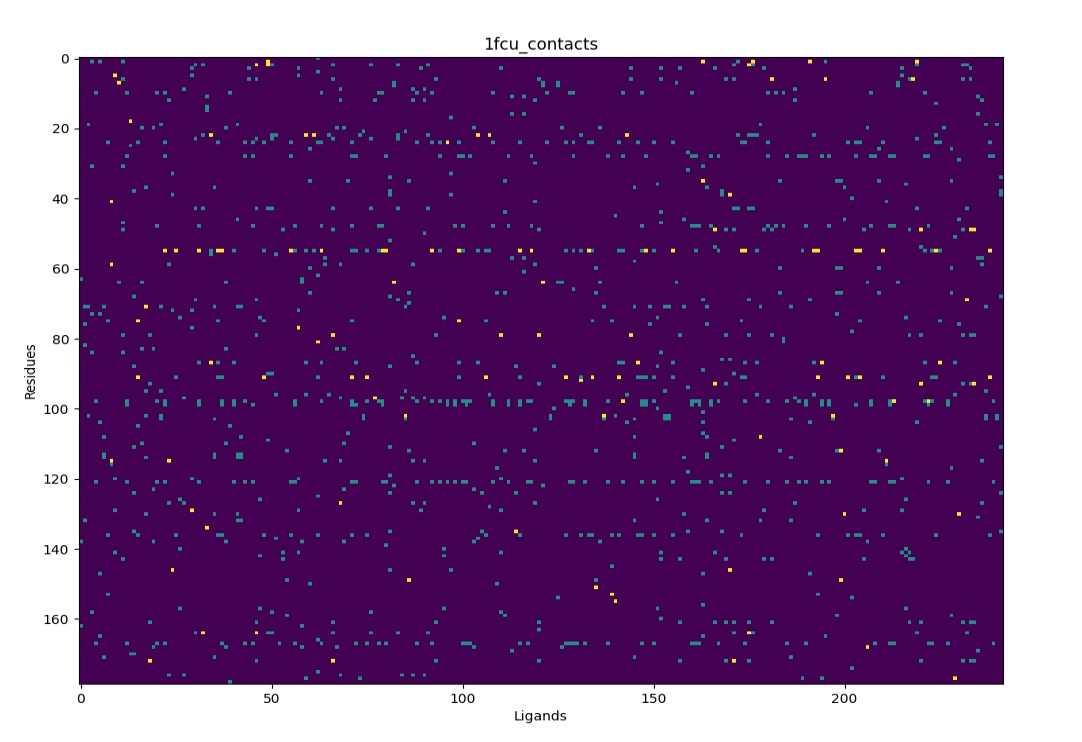
\includegraphics[width=\textwidth, height=6cm]{images/chapter4/heatmaps/heatmap_gnina_1fcu.jpg}
        \caption[]%
        {{\small Heatmap delle interazioni per la proteina 1FCU prodotta a partire dalle pose predette dei ligandi da GNINA.}}    
        \label{fig:heatmap_gnina_1fcu}
    \end{subfigure}
    \hfill
    \begin{subfigure}[b]{\textwidth}  
        \centering 
        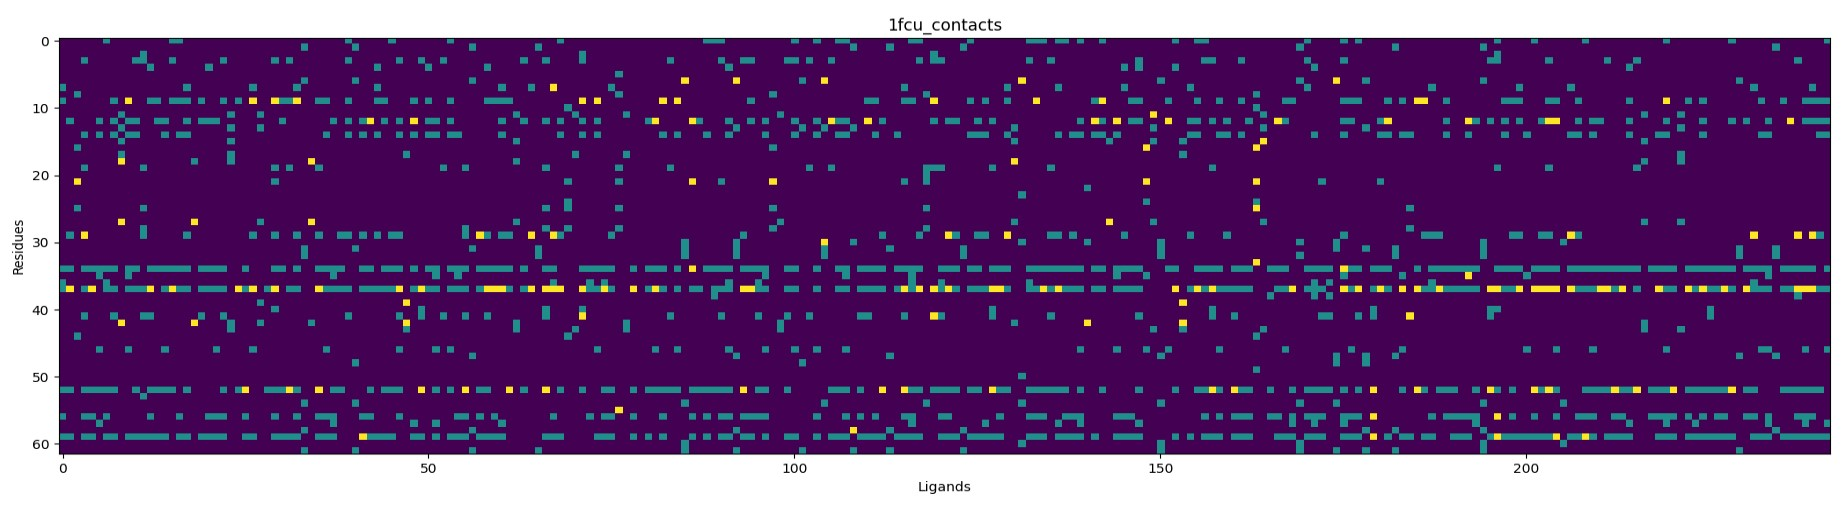
\includegraphics[width=0.9\textwidth, height=6cm]{images/chapter4/heatmaps/heatmap_vina_1fcu.jpg}
        \caption[]%
        {{\small Heatmap delle interazioni per la proteina 1FCU prodotta a partire dalle pose predette dei ligandi da AutoDock Vina.}}    
        \label{fig:heatmap_vina_1fcu}
    \end{subfigure}
    \caption[Visualizzazione delle heatmaps per la proteina 1FCU.]
    {\small Visualizzazione delle interazioni per la proteina 1FCU attraverso heatmaps. In alto, è riportata l'heatmap risultante dalle pose predette da GNINA mentre in basso, quella risultante dalle pose predette da AutoDock Vina. Sull'asse delle ascisse sono riportati i ligandi, sulle ordinate i residui coinvolti per la proteina. In giallo sono riportati i legami a idrogeno, in azzurro/verde i close contacts, in viola nessun legame. } 
    \label{fig:1fcu}
\end{figure}
 
La Figura \ref{fig:1fcu} riporta le heatmaps prodotte dall'analisi delle interazioni molecolari relativamente alla proteina 1FCU per il dataset dei ligandi utilizzato (vedi Figura \ref{fig:heatmap_gnina_1fcu} per GNINA, vedi \ref{fig:heatmap_vina_1fcu} per AutoDock Vina).

Sebbene proteine e ligandi siano processati pedissecuamente e forniti in input ai due software, come già anticipato dalla Tabella \ref{contacts_table} in termini qualitativi e quantitativi, le interazioni molecolari prodotte all'interno del complesso sono profondamente diverse. La visualizzazione delle heatmaps permette una conferma di quanto detto. 
Analizzando la Figura \ref{fig:heatmap_gnina_1fcu} che è relativa ai risultati di GNINA, è possibile notare come i residui coinvolti nell'intero processo superino le 100 unità, presentando inoltre una distribuzione più equa dei legami all'interno del complesso. Infatti, risulta impensabile cercare di sintetizzare le interazioni molecolari per la proteina 1FCU semplicemente attraverso un sotto-insieme di residui che la compongono.

La situazione è completamente diversa nel caso dei risultati di AutoDock Vina: in primo luogo, poiché il numero di residui coinvolti è pari a circa 60 unità; in secondo luogo, nell'heatmap stessa, sebbene le interazioni siano maggiori in numero,  queste sono maggiormente concentrate in determinati residui (ARG244, SER225, TYR188, TYR190). In altre parole, se nel caso di GNINA, ciascun residuo fornisce il proprio contributo in termini di interazioni, nel caso di AutoDock Vina, siamo in grado di discernere dall'insieme dei residui coinvolti, i residui che forniscono l'apporto maggiore al numero di interazioni e quelli che invece hanno un contributo minimo. Questo tipo di considerazione può essere interessante per traslare l'analisi in siti proteici specifici, ovvero quelli in cui risiedono i residui principali, piuttosto che di blind docking come nel nostro caso.

Questo tipo di situazione appare ancora più netta nel caso della proteina 5XZ3\_A, prendendo visione della Figura \ref{fig:5xz3_a}. 

\begin{figure}
    \centering
    \begin{subfigure}[b]{\textwidth}
        \centering
        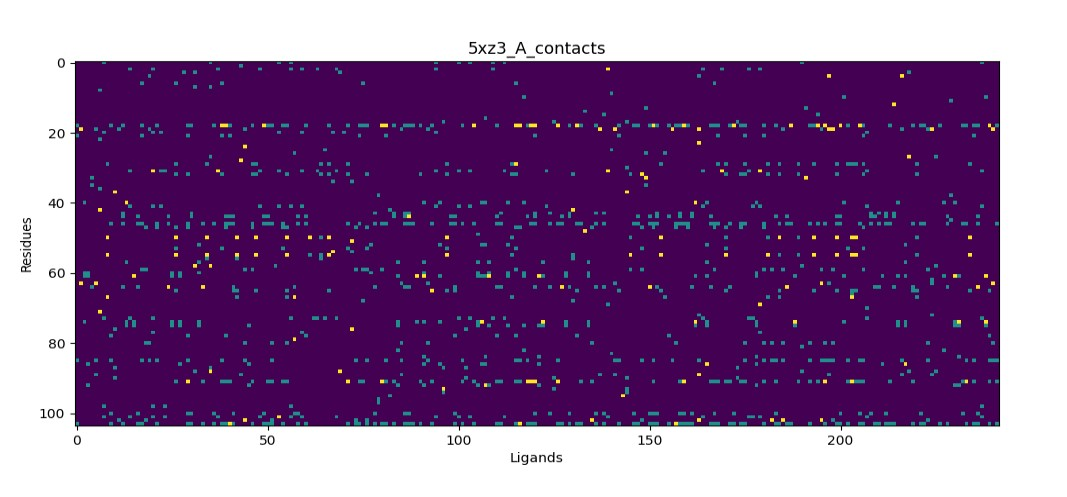
\includegraphics[width=\textwidth, height=6cm]{images/chapter4/heatmaps/heatmap_gnina_5xz3_a.jpg}
        \caption[]%
        {{\small Heatmap delle interazioni per la proteina 5XZ3\_A prodotta a partire dalle pose predette dei ligandi da GNINA.}}    
        \label{fig:heatmap_gnina_5xz3_a}
    \end{subfigure}
    \hfill
    \begin{subfigure}[b]{\textwidth}  
        \centering 
        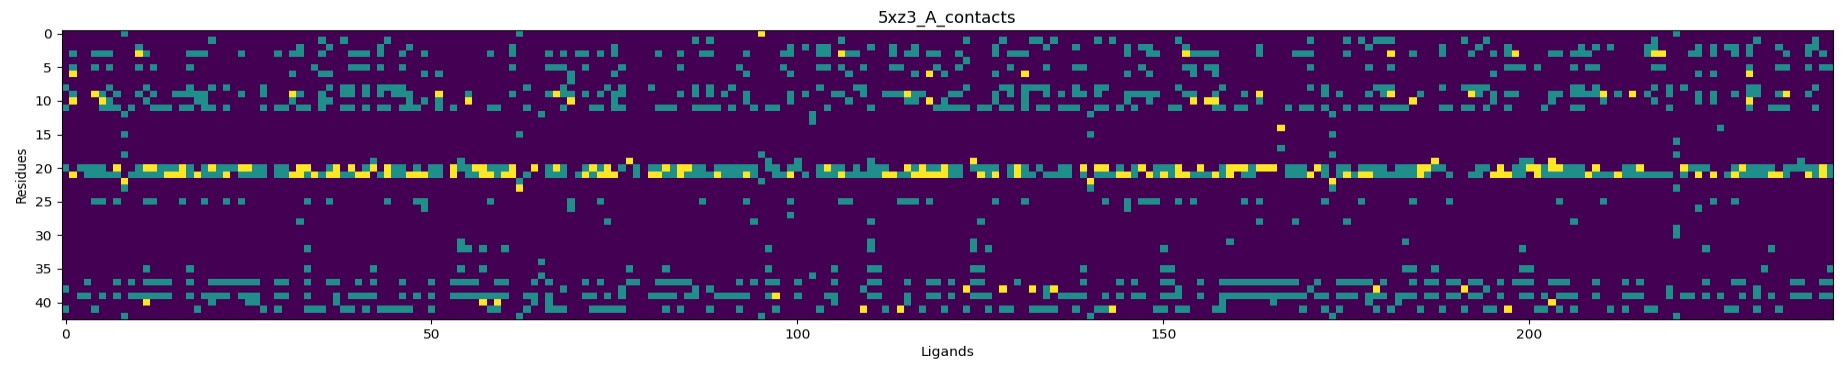
\includegraphics[width=0.9\textwidth, height=3cm]{images/chapter4/heatmaps/heatmap_vina_5xz3_a.jpg}
        \caption[]%
        {{\small Heatmap delle interazioni per la proteina 5XZ3\_A prodotta a partire dalle pose predette dei ligandi da AutoDock Vina.}}    
        \label{fig:heatmap_vina_5xz3_a}
    \end{subfigure}
    \caption[Visualizzazione delle heatmaps per la proteina 5XZ3\_A.]
    {\small Visualizzazione delle interazioni per la proteina 5XZ3\_A attraverso heatmaps. In alto, è riportata l'heatmap risultante dalle pose predette da GNINA mentre in basso, quella risultante dalle pose predette da AutoDock Vina. Sull'asse delle ascisse sono riportati i ligandi, sulle ordinate i residui coinvolti per la proteina. In giallo sono riportati i legami a idrogeno, in azzurro/verde i close contacts, in viola nessun legame. } 
    \label{fig:5xz3_a}
\end{figure}

In questo caso però, la particolarità delle relative heatmaps sta nel fatto che nel caso della Figura \ref{fig:heatmap_vina_5xz3_a}, corrispondente ai risultati di AutoDock Vina, è possibile sintetizzare non solo la maggior parte delle interazioni in un sotto-insieme dei residui coinvolti, comunque minore in numero rispetto a quello evidenziato dalla Figura \ref{fig:heatmap_gnina_5xz3_a} relativa ai risultati di GNINA, ma anche la maggior parte dei legami a idrogeno prodotti in un sotto-insieme ancor più ridotto dei residui che compongono la proteina (HIS61, TYR72).

Sebbene le considerazioni siano plausibili nel caso di AutoDock Vina, rispetto al caso di GNINA queste sono totalmente insignificanti.

Le medesime considerazioni possono essere fatte ancor più intuitivamente visualizzando gli istogrammi relativi alle interazioni prodotte, i cui picchi individuano i residui maggiormente presenti nei legami. In basso sono riportati i residui che effettuano almeno un'interazione rilevanti; in blu è riportato il numero di close contacts mentre in arancione il numero di legami a idrogeno per ciascun residuo proteico.

\begin{figure}
    \centering
    \begin{subfigure}[b]{\textwidth}
        \centering
        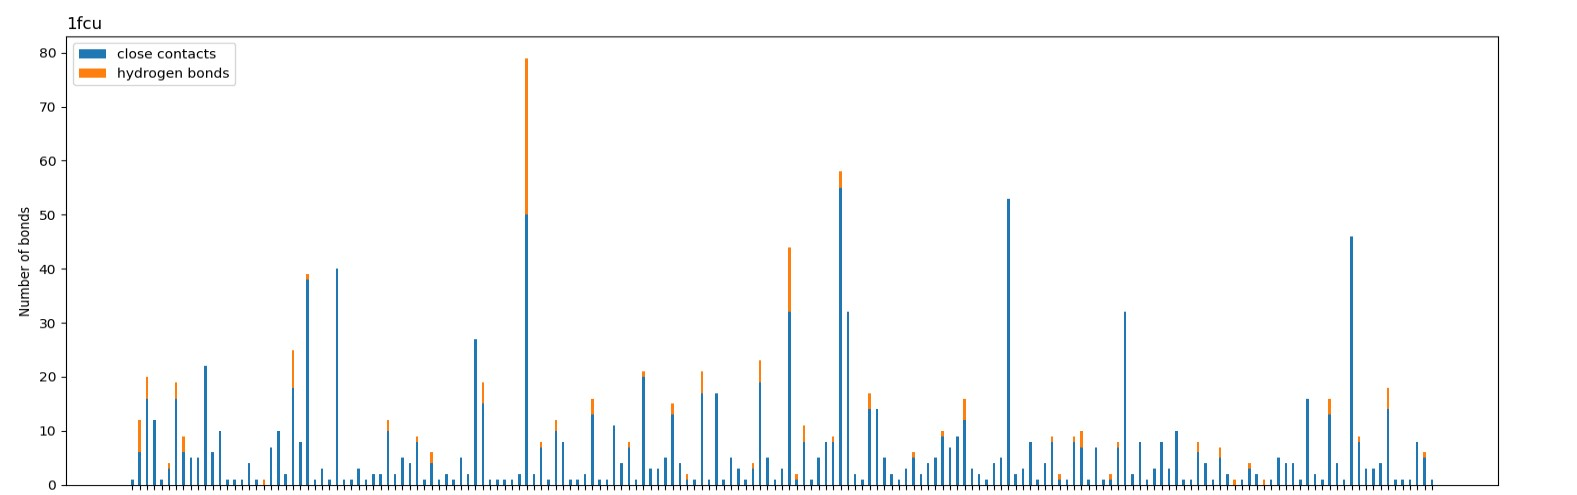
\includegraphics[width=\textwidth, height=6cm]{images/chapter4/interactions/interactions_gnina_1fcu.jpg}
        \caption[]%
        {{\small Heatmap delle interazioni per la proteina 5XZ3\_A prodotta a partire dalle pose predette dei ligandi da GNINA.}}    
        \label{fig:interactions_gnina_1fcu}
    \end{subfigure}
    \hfill
    \begin{subfigure}[b]{\textwidth}  
        \centering 
        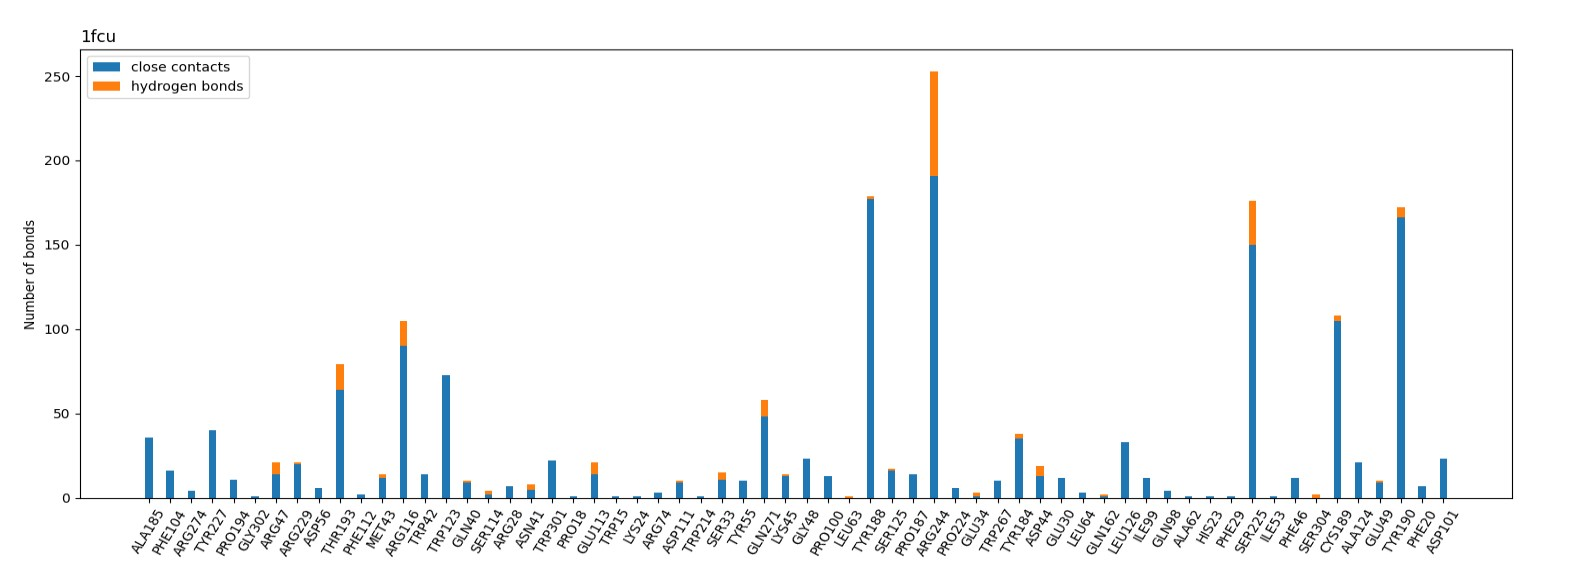
\includegraphics[width=0.9\textwidth, height=3cm]{images/chapter4/interactions/interactions_vina_1fcu.jpg}
        \caption[]%
        {{\small Istogramma delle interazioni per la proteina 1FCU prodotta a partire dalle pose predette dei ligandi da AutoDock Vina.}}    
        \label{fig:interactions_vina_1fcu}
    \end{subfigure}
    \caption[Visualizzazione degli istogrammi per la proteina 1FCU.]
    {\small Visualizzazione delle interazioni per la proteina 1FCU attraverso istogrammi. In alto, è riportato l'istogramma risultante dalle pose predette da GNINA mentre in basso, quello risultante dalle pose predette da AutoDock Vina. Sull'asse delle ordinate è riportato il numero di contatti, sulle ascisse i residui coinvolti per ciascuna proteina. In arancione sono riportati i legami a idrogeno, in blu i close contacts. } 
    \label{fig:int_1fcu}
\end{figure}


\begin{figure}
    \centering
    \begin{subfigure}[b]{\textwidth}
        \centering
        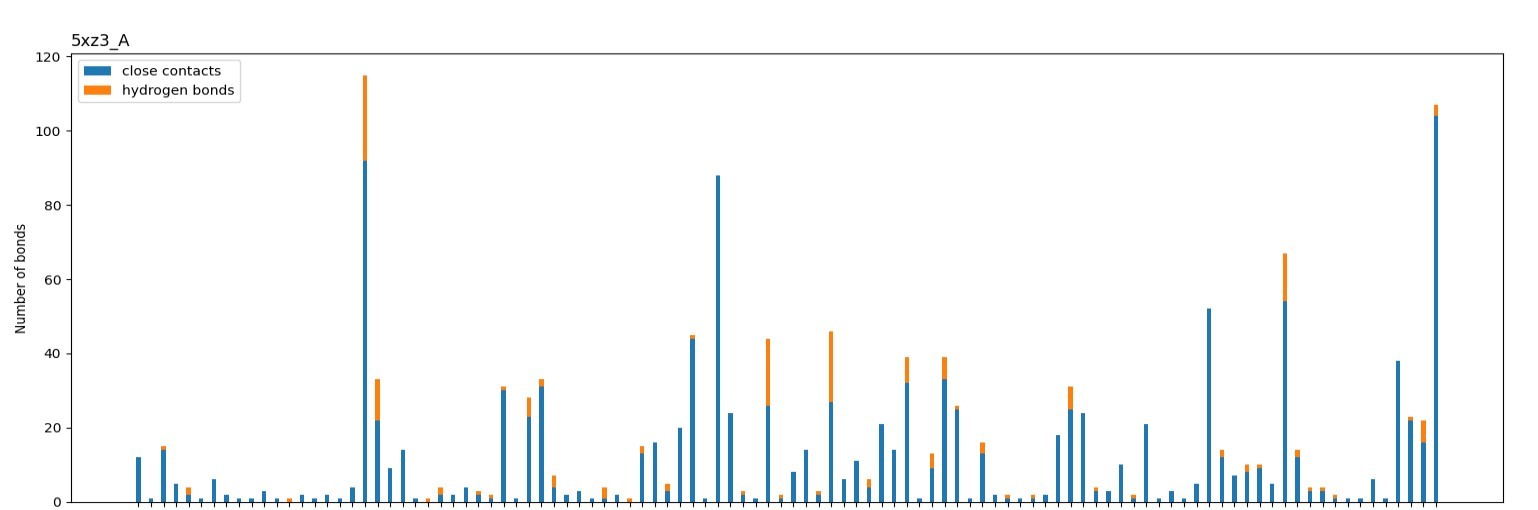
\includegraphics[width=\textwidth, height=6cm]{images/chapter4/interactions/interactions_gnina_5xz3_a.jpg}
        \caption[]%
        {{\small Istogramma delle interazioni per la proteina 5XZ3\_A prodotta a partire dalle pose predette dei ligandi da GNINA.}}    
        \label{fig:interactions_gnina_5xz3_a}
    \end{subfigure}
    \hfill
    \begin{subfigure}[b]{\textwidth}  
        \centering 
        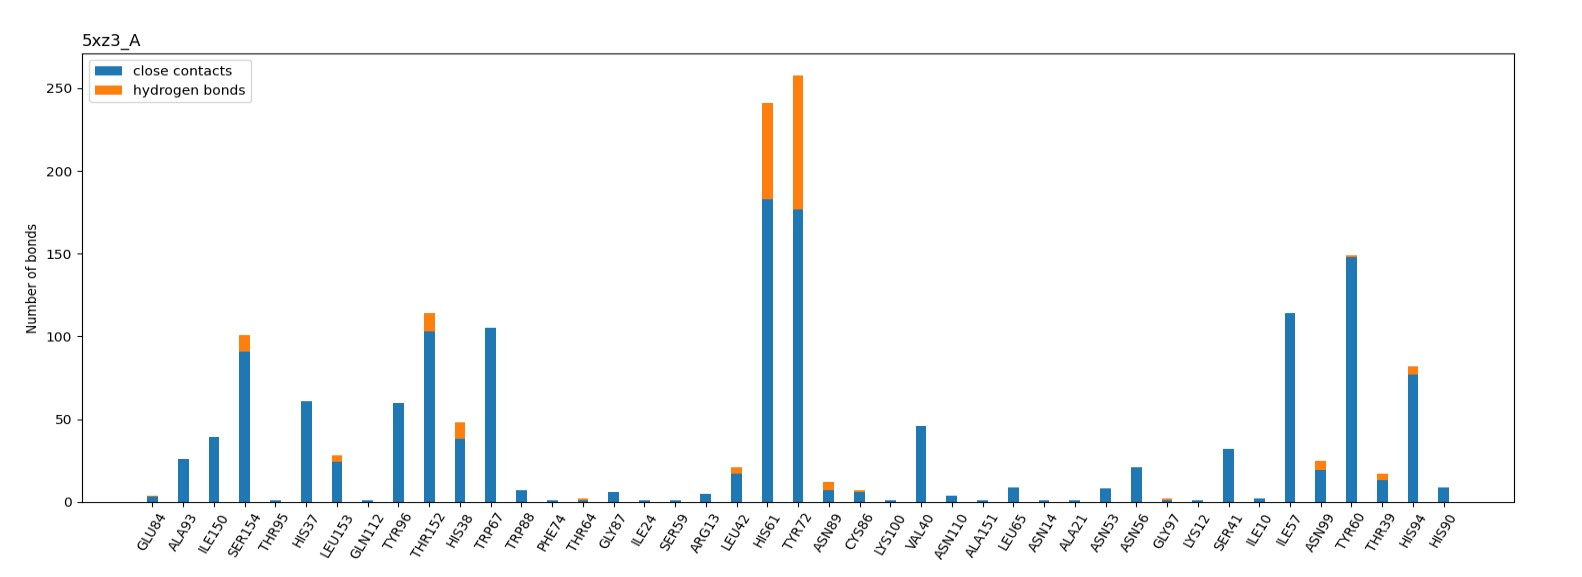
\includegraphics[width=0.9\textwidth, height=3cm]{images/chapter4/interactions/interactions_vina_5xz3_a.jpg}
        \caption[]%
        {{\small Istogramma delle interazioni per la proteina 5XZ3\_A prodotta a partire dalle pose predette dei ligandi da AutoDock Vina.}}    
        \label{fig:interactions_vina_5xz3_a}
    \end{subfigure}
    \caption[Visualizzazione degli istogrammi per la proteina 5XZ3\_A.]
    {\small Visualizzazione delle interazioni per la proteina 5XZ3\_A attraverso istogrammi. In alto, è riportato l'istogramma risultante dalle pose predette da GNINA mentre in basso, quello risultante dalle pose predette da AutoDock Vina. Sull'asse delle ordinate è riportato il numero di contatti, sulle ascisse i residui coinvolti per ciascuna proteina. In arancione sono riportati i legami a idrogeno, in blu i close contacts.} 
    \label{fig:int_5xz3_a}
\end{figure}

Mettendo insieme queste considerazioni, assieme a quelle fatte in precedenza all'interno di questo capitolo, siamo in grado di affermare che le prestazioni della rete neurale convoluzionale applicata all'interno di GNINA danno luogo a risultati estremamente diversi rispetto a quelli forniti da un software tradizionalmente usato per analisi di blind docking. 
In particolare, dall'analisi dei risultati sperimentali emerge che le predizioni effettuate da GNINA risultano essere migliori in termini di RMSD (vedi Tabella \ref{rmsd_table}) ma peggiori in termini di affinità (vedi Tabella \ref{affinity_table}). Dal punto di vista delle interazioni molecolari nel complesso però è stato dimostrato che, sebbene siano quantitativamente inferiori, queste siano qualitativamente migliori, come testimonia la parità rispetto all'Hydrogen Bonds Ratio (vedi Tabella \ref{contacts_table}).

Ciò significa che una bassa RMSD non implica necessariamente un'affinità migliore e che un'affinità migliore non implica necessariamente legami più stabili ed efficaci. 

Nonostante il numero di legami sia inferiore, è emerso che il numero di residui coinvolti in legami è notevolmente maggiore, producendo quindi heatmaps più ampie e sparse in cui le interazioni sono maggiormente distribuite, rispetto a quelle ridotte e fitte di AutoDock Vina, in cui è maggiormente possibile approssimare l'insieme dei residui coinvolti in interazioni ad un sotto-insieme ridotto di residui interessanti.



\section{Considerazioni sui tempi del docking}
% confronto sui tempi/prestazioni
La durata dell'intero processo di docking è estremamente lunga ed è influenzata dalla dimensione del dataset iniziale che si vuole analizzare e dalle risorse a disposizione. Nonostante lo sfruttamento di ambienti di calcolo parallelo, rimane comunque un'operazione onerosa sia dal punto di vista computazionale sia in termini di risorse impiegate. 

L'utilizzo della rete neurale convoluzionale costringe all'impiego di moderne risorse hardware per compiere il processo di docking sottoposto. 
Ragion per cui, è necessaria almeno una moderna GPU NVIDIA con 4 o più GB di RAM per avere risultati in tempi moderati \cite{mcnutt_gnina_2021}. 

Per l'ottenimento dei risultati relativi alle proteine selezionate, sono state necessarie in media circa 3 ore, sfruttando le potenze di calcolo messe a disposizione da Google Colab. 
In generale l'ottenimento dei risultati per entrambi i software ha richiesto circa lo stesso tempo; tuttavia, nel caso di GNINA, sono state utilizzate risorse hardware importanti, rappresentando un aspetto da non trascurare assolutamente nella scelta del software di docking per l'analisi che si vuole effettuare. Il tempo impiegato dal software, e quindi dall'applicazione delle rete neurale convoluzionale all'interno del processo di docking, e la necessità di una potenza di calcolo modesta rappresentano le maggiori criticità dell'approccio avanzato. L'elaborato è la dimostrazione di come grazie al 
\textbf{cloud computing} sia possibile, in parte, far fronte a tali criticità.

